\chapter{Tools} 
Multiple tools were used in the process of creating the demo application for
this paper including the Unity game engine, Blender as a modeling and animation
software, and MakeHuman as a model creation tool. This chapter discusses the
built-in functionalities which make the mentioned tools an effective choice.

\section{MakeHuman}
MakeHuman is an open source tool for making 3D characters. It provides
a convenient way of acquiring a human model which is customizable and can be
exported in various formats in order to be used in other software programs. The
key factors which make this tool suitable for use in the demo application is the
options it provides regarding the complexity of the topology of the model's
mesh, and the choice of skeleton rig alongside the fact that the exported model
is already rigged and ready to be used in an animation software. One of the rig
options is specifically designed to be then used in a game engine setting
(Figure \ref{fig:mh_rig}).

\begin{figure}
    \centering
    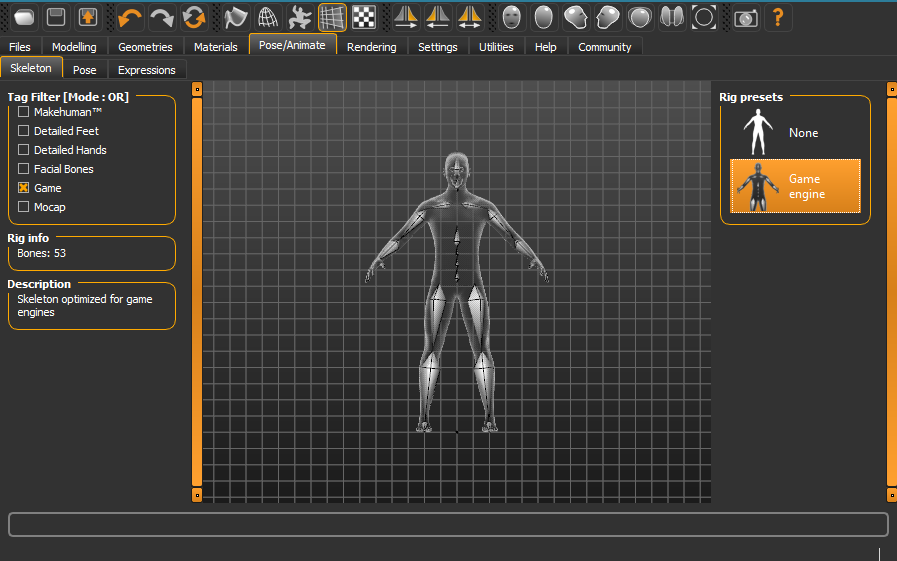
\includegraphics[width=\textwidth]{grafika/make_human_rig.png}
    \caption{MakeHuman rig selection}
    \label{fig:mh_rig}
\end{figure}

\section{Blender}
The tool of choice for modeling and animation used for the demo application is
Blender. It is a free and open source tool offering a suite of functionalities
including the creation of 3D models, rigging, and animation. 

% The program enables
% users to import models in various formats, which allows the user to use
% externally generated models, such as the ones created in MakeHuman, and animate
% them. 

Blender offers the functionality of importing existing models in various formats
including the \textit{collada} format \cite{collada} which is the default export
option in MakeHuman. The models, which are already rigged, can then be animated
using the Blender animation pose editor. 

Models can also be created from scratch. Blender offers a 3D modelling tool to
create a desired mesh. A custom rig can also be constructed and attached to the
created model. Weights can be painted on the meshes vertices for each bone to
define how tightly they are bound, and how much the position of each vertex
depends on the given bone position. 

Lastly, an animation sequence can be created for an existing mesh and rig using
the character animation pose editor. The user can define poses for different
points in time by creating key frames on a timeline, and blender interpolates the
bone positions in between the key frames. This is used to create baked animations
for characters and objects, as well as defining animations that are later
blended with IK constraints. An animated model can be then exported in the
\textit{fbx} format to be used in other software programs. Unity also supports
importing a model from a \textit{.blend} file which is the extension of
a blender project file. 


\section{Unity}
The Unity game engine is the one tool which was non-negotiable as the paper
is meant to specifically focus on the usage of inverse kinematics in said game
engine. Nevertheless, the engine is a good selection for this use case due to
its advanced 3D support, the built-in packages and functionalities which are
geared towards the subject of this paper, and the overall popularity of the
engine and large community built around it which results in a substantial amount
of documentation and support. 

\subsection{Importing Animations}

\subsection{Animator Controller}

\subsection{Animation Rigging Package}
